\documentclass{beamer}

\mode<presentation>
{
  \usetheme{Boadilla}      
  \usecolortheme{dove} 
  \usefonttheme{structurebold}  
  \setbeamertemplate{navigation symbols}{}
  \setbeamertemplate{caption}[numbered]
} 

\usepackage[english]{babel}
\usepackage[utf8x]{inputenc}
\usepackage{fancybox}
\usepackage{tikz}
\usetikzlibrary{arrows,shapes}

\setbeamertemplate{itemize item}{\scriptsize\raise1.25pt\hbox{\donotcoloroutermaths$\blacktriangleright$}}
\setbeamertemplate{itemize subitem}{\tiny\raise1.5pt\hbox{\donotcoloroutermaths$\blacktriangleright$}}
\setbeamertemplate{itemize subsubitem}{\tiny\raise1.5pt\hbox{\donotcoloroutermaths$\blacktriangleright$}}
\setbeamertemplate{enumerate item}{\insertenumlabel.}
\setbeamertemplate{enumerate subitem}{\insertenumlabel.\insertsubenumlabel}
\setbeamertemplate{enumerate subsubitem}{\insertenumlabel.\insertsubenumlabel.\insertsubsubenumlabel}
\setbeamertemplate{enumerate mini template}{\insertenumlabel}

\setbeamertemplate{section in toc}{%
  {\usebeamercolor[fg]{title}\inserttocsectionnumber.}~\inserttocsection}
\setbeamercolor{subsection in toc}{bg=white,fg=structure}
\setbeamertemplate{subsection in toc}{%
  \hspace{1.2em}{\usebeamercolor[fg]{title}\rule[0.3ex]{3pt}{3pt}}~\inserttocsubsection\par}

\defbeamertemplate*{title page}{customized}[1][]
{
  \usebeamerfont{title}\inserttitle\par
  \usebeamerfont{subtitle}\usebeamercolor[fg]{subtitle}\insertsubtitle\par
  \bigskip
  \usebeamerfont{author}\insertauthor\par
  \usebeamerfont{institute}Department of Physics and Astronomy\par
  \usebeamerfont{institute}George Mason University, Fairfax, VA\par
  \bigskip
  \usebeamerfont{date}\insertdate\par

}
\title[ECA w/ time series causality]{Exploratory Causal Analysis in Bivariate Time Series Data}
\author{J.\ M.\ McCracken}
\institute{GMU}
\date{\today}

\begin{document}
\tikzstyle{every picture}+=[remember picture]
\everymath{\displaystyle}


\begin{frame}
  \titlepage
\end{frame}

% Uncomment these lines for an automatically generated outline.
\begin{frame}{Outline}
 \tableofcontents
\end{frame}

\section{Causality studies}
\begin{frame}{Causality studies}
\begin{block}{The study of causality is as old as science itself }
\begin{itemize}
\item \vfill Modern historians credit Aristotle with both the first theory of causality (``four causes'') and an early version of the scientific method
\note[item]{the material cause, the formal cause, the efficient cause, and the final cause}
\item \vfill The modern study of causality is broadly interdisciplinary; far too broad to review in a short talk.
\end{itemize}
\end{block}
\vspace{1cm}
Illari and Russo's textbook\footnotemark provides an overview of causality studies
\note{This book focuses on philosophical causality studies, but I have not found a modern books that provides the same breadth of coverage or condenses the salient points as well.}
\footnotetext[1]{{\tiny Illari, P., \& Russo, F. (2014). Causality: Philosophical theory meets scientific practice. Oxford University Press.}}
\end{frame}

\begin{frame}{Towards a taxonomy of causal studies}
Paul Holland identified four types of causal questions\footnotemark:
\begin{itemize}
\item \alert<2>{the ultimate meaningfulness of the notion of causality}
\item \alert<2>{the details of causal mechanisms}
\item \alert<3>{the causes of a given effect}
\item \alert<3>{the effects of a given cause}
\end{itemize}
\pause
\vspace{0.25in}
\alert<2>{Foundational causality} ``Is a cause required to precede an effect?'' or  ``How are causes and effects related in space-time?''
\pause
\vspace{0.25in}

\alert<3>{Data causality} ``Does smoking cause lung cancer?'' or  ``Are traffic accidents caused by rain storms?''

\footnotetext[2]{{\tiny Holland, P. W. (1986). Statistics and causal inference. Journal of the American statistical Association, 81(396), 945-960.}}
\end{frame}

\section{Data causality}
\begin{frame}{Data causality}
\fbox{Data causality is data analysis to draw causal inferences}
\vspace{0.25in}

\pause
Approaches to data causality studies include
\begin{itemize}
\item design of experiments (e.g., Fisher randomization)
\note[item]{This is still considered the ``gold standard'' for causal inference; i.e., many authors consider experiments with Fisher randomization to be the only way to draw causal inference from data.}
\pause
\item potential outcomes (Rubin's counterfactuals)
\note[item]{This is perhaps the most popular approach to data causality in the social and medical sciences.}
\pause
\item directed acyclic graphs (DAGs) with structural equation models (SEMs); popularized by Pearl as ``structural causal models (SCMs)''
\note[item]{Pearl has stated that SCM should replace all other data causality approaches.}
\pause
\item \alert<7>{time series causality}
\end{itemize}
\pause
\begin{block}{There is no consensus on the best approach to data causality}
Many authors consider their favored approach to be the exclusive {\em correct} approach.  
\end{block}
\end{frame}

\begin{frame}{Time series causality}
\fbox{Time series causality is data causality with time series data}
\vspace{0.25in}
\pause

Approaches to time series causality can be roughly divided into five categories,
\begin{itemize}
\item Granger (model based approaches)
\item Information-theoretic 
\item State space reconstruction (SSR)
\item Correlation 
\item Penchant
\end{itemize}

\end{frame}

\section{Exploratory causal analysis}
\begin{frame}{Exploratory causal analysis}
\framesubtitle{Language}

{\bf Exploring} causal structures in data sets is distinct from {\bf confirming} causal structures in data sets.
\vspace{0.25in}

Causal language used in ECA should not be conflated with other typical uses; i.e., ``cause'', ``effect'', ``drive'', etc.\ are used as technical terms with definitions unrelated to their common, everyday definitions.
\vspace{0.25in}
\pause

$\rightarrow$ and $\leftarrow$ will be used as shorthand for causal statements,

e.g., $A$ drives $B$ will be written as $A\rightarrow B$.
\end{frame}

\begin{frame}{Exploratory causal analysis}
\framesubtitle{Assumptions}

\begin{block}{A cause always precedes an effect.}
This assumption is required for the operational definitions of causality.
\end{block}
\vspace{0.5in}

\begin{block}{A driver may be present in the data being analyzed.}
This assumption may lead to issues of confounding.
\end{block}

\note{These are not the only assumptions, but they are the most important for creating operational definitions of causality.  The other assumptions, including measurements do not change the system, measurements across equivalent systems are comparable, systems are comparable across different points in time, etc., are assumptions common to most experimental physics and not necessarily related to causality.}
\end{frame}

\begin{frame}{Exploratory causal analysis}
\framesubtitle{ECA guess vector approach}

We will not favor a specific operational definition of causality $\Rightarrow$ we do not favor any particular tool

\vspace{0.25in}
Consider a time series pair $(\mathbf{X},\mathbf{Y})$,
\pause

\begin{block}{ECA guess vector}
Define a vector $\vec{g}$ where each element $g_i$ is defined as either 0 if $\mathbf{X}\rightarrow\mathbf{Y}$, 1 if $\mathbf{X}\leftarrow\mathbf{Y}$, or 2 if no causal inference can be made.  The value of each $g_i$ comes from a specific time series causality tool.
\end{block}
\pause
\begin{block}{ECA guess }
The {\em ECA guess} is either $\mathbf{X}\rightarrow\mathbf{Y}$, $\mathbf{Y}\rightarrow\mathbf{X}$, or undefined, with $g_i = 0\;\forall g_i\in\vec{g}\Rightarrow\mathbf{X}\rightarrow\mathbf{Y}$ and $g_i = 1\;\forall g_i\in\vec{g}\Rightarrow\mathbf{Y}\rightarrow\mathbf{X}$.
\end{block}
\end{frame}

\section{Making an ECA guess}
\begin{frame}{Making an ECA guess}
Our focus is on time series, so each causal inference $g_i\in \vec{g}$ will be drawn from a tool in one of each of the five time series causality categories.

\note{The decision to use one tool in each category was meant to keep the length of $\vec{g}$ manageable while providing a wide variety in the operational definitions of causality.}
\pause

\vspace{0.25in}
\begin{columns}
\column{0.15\textwidth}
\only<3>{\textbullet}\hfill $g_1$\\
\only<4>{\textbullet}\hfill $g_2$\\
\only<5>{\textbullet}\hfill $g_3$\\
\only<6>{\textbullet}\hfill $g_4$\\
\only<7>{\textbullet}\hfill $g_5$
\column{0.85\textwidth}
\alert<3->{transfer entropy difference} \only<3->{information-theoretic}\\
\alert<4->{Granger log-likelihood statistics} \only<4->{Granger}\\
\alert<5->{pairwise asymmetric inference (PAI)} \only<5->{SSR}\\
\alert<6->{average weighted mean observed leaning} \only<6->{penchant}\\
\alert<7->{lagged cross-correlation difference} \only<7->{correlation}
\end{columns}
\end{frame}

\subsection{Transfer entropy difference}
\begin{frame}{Transfer entropy ($g_1$)}
\framesubtitle{Shannon entropy}
\tikzstyle{na} = [baseline=-.5ex]

The uncertainty that a random variable $\mathbf{X}$ takes some specific value $X_n$ is given by the Shannon (or information) entropy,
\only<1>{\begin{equation*}
H_X = -\sum_{n=1}^{N_X} P(\mathbf{X}=X_n) \log_2 P(\mathbf{X}=X_n)
\end{equation*}}
\only<2>{\begin{equation*}
H_X = -\sum_{n=1}^{N_X} 
			\tikz[baseline]{
            \node[fill=blue!20,anchor=base] (t1a)
            {$P(\mathbf{X}=X_n)$}
            }
            \log_2 
            \tikz[baseline]{
            \node[fill=blue!20,anchor=base] (t1b)
            {$P(\mathbf{X}=X_n)$}
            }
\end{equation*}}
\only<3>{\begin{equation*}
H_X = -\tikz[baseline]{
            \node[fill=blue!20,anchor=base] (t2)
            {$\sum_{n=1}^{N_X}$}
            }
            P(\mathbf{X}=X_n) \log_2 P(\mathbf{X}=X_n)
\end{equation*}}
\only<4>{\begin{equation*}
H_X = -\sum_{n=1}^{N_X} P(\mathbf{X}=X_n)
			\tikz[baseline]{
            \node[fill=blue!20,anchor=base] (t3)
            {$\log_2$}
            }
            P(\mathbf{X}=X_n)
\end{equation*}}
\only<2,3,4>{\vspace{0.25in}}
\begin{center}
\only<2>{
\tikz[na] \node[coordinate] (n1) {};

$P(\mathbf{X}=X_n)$ is the probability that $\mathbf{X}$ takes the specific value $X_n$}
\only<3>{
\tikz[na] \node[coordinate] (n2) {};

The sum is over all possible values of $X_n$; $n=1,2,\ldots, N_X$}
\only<4>{
\tikz[na] \node[coordinate] (n3) {};

The base of the logarithm sets the entropy units, which is ``bits'' here}
\end{center}

\only<2>{
\begin{tikzpicture}[overlay]
        \path[->]<1-> (n1) edge [bend right=10] (t1b);
        \path[->]<1-> (n1) edge [bend left=10] (t1a);
\end{tikzpicture}}
\only<3>{
\begin{tikzpicture}[overlay]
        \path[->]<1-> (n2) edge [bend left=10] (t2);
\end{tikzpicture}}
\only<4>{
\begin{tikzpicture}[overlay]
        \path[->]<1-> (n3) edge [bend right=10] (t3);
\end{tikzpicture}}
\end{frame}

\begin{frame}{Transfer entropy ($g_1$)}
\framesubtitle{Shannon entropy example}

\begin{exampleblock}{Binary example (to help with intuition)}
Consider a coin $\mathbf{C}$ that take the value $H$ with probability $p_H$ and $T$ with probability $p_T$.  The Shannon entropy is 
\begin{equation*}
H_C = -\left(p_H\log_2 p_H + p_T\log_2 p_T\right)
\end{equation*}
\pause
\hfill\\
\alert{completely uncertain of outcome}\\
\hspace{0.1in} Fair coin $\Rightarrow p_H=p_T=0.5\Rightarrow H_C = 1$\\
\pause
\hfill\\
\alert{completely certain of outcome}\\
\hspace{0.1in} Always heads (or tails) $\Rightarrow p_{H(T)}=0,p_{T(H)}=1\Rightarrow H_C = 0$\\
\end{exampleblock}
\pause
{\small (Entropy calculations almost always assume $0\log_2 0 := 0$.)}
\end{frame}

\begin{frame}{Transfer entropy ($g_1$)}
\framesubtitle{Mutual information}
\tikzstyle{na} = [baseline=-.5ex]

A pair of random variables $(\mathbf{X},\mathbf{Y})$ have some mutual information given by
\only<1,4->{\begin{eqnarray*}
I_{X;Y} &=& H_X + H_Y - H_{X,Y}\\ 
&=& \sum_{n=1}^{N_X} \sum_{m=1}^{N_Y} P(\mathbf{X}=X_n,\mathbf{Y}=Y_m) \log_2 \frac{P(\mathbf{X}=X_n,\mathbf{Y}=Y_m)}{P(\mathbf{X}=X_n)P(\mathbf{Y}=Y_m)}
\end{eqnarray*}}

\only<2>{\begin{eqnarray*}
I_{X;Y} &=& H_X + H_Y - H_{X,Y}\\ 
&=& \sum_{n=1}^{N_X} \sum_{m=1}^{N_Y} 
	\tikz[baseline]{
            \node[fill=blue!20,anchor=base] (t1)
            {$P(\mathbf{X}=X_n,\mathbf{Y}=Y_m)$}
            }\log_2 \frac{P(\mathbf{X}=X_n,\mathbf{Y}=Y_m)}{P(\mathbf{X}=X_n)P(\mathbf{Y}=Y_m)}
\end{eqnarray*}}

\only<3>{\begin{eqnarray*}
I_{X;Y} &=& H_X + H_Y - H_{X,Y}\\ 
&=& \sum_{n=1}^{N_X} \sum_{m=1}^{N_Y} P(\mathbf{X}=X_n,\mathbf{Y}=Y_m) \log_2
	\tikz[baseline]{
            \node[fill=blue!20,anchor=base] (t2)
            {$\frac{P(\mathbf{X}=X_n,\mathbf{Y}=Y_m)}{P(\mathbf{X}=X_n)P(\mathbf{Y}=Y_m)}$}}
\end{eqnarray*}}
\only<2-4>{\vspace{0.25in}}

\begin{center}
\only<2>{
\tikz[na] \node[coordinate] (n1) {};

$P(\mathbf{X}=X_n,\mathbf{Y}=Y_m)$ is the probability that $\mathbf{X}$ takes the specific value $X_n$ and $\mathbf{Y}$ takes the specific value $Y_m$}
\only<3>{
\tikz[na] \node[coordinate] (n2) {};

If $\mathbf{X}$ and $\mathbf{Y}$ are independent, then $P(\mathbf{X}=X_n,\mathbf{Y}=Y_m)=P(\mathbf{X}=X_n)P(\mathbf{Y}=Y_m)\Rightarrow I_{X;Y} = 0$}

\only<4>{\fbox{The mutual information is symmetric; i.e., $I_{X;Y}=I_{Y;X}$}}
\end{center}

\only<5>{Schreiber proposed an extension of the mutual information to measure ``information flow'' by making it conditional and including assumptions about the temporal behavior $\mathbf{X}$ and $\mathbf{Y}$.}

\only<2>{
\begin{tikzpicture}[overlay]
        \path[->]<1-> (n1) edge [bend left=10] (t1);
\end{tikzpicture}}
\only<3>{
\begin{tikzpicture}[overlay]
        \path[->]<1-> (n2) edge [bend right=10] (t2);
\end{tikzpicture}}
\end{frame}

\begin{frame}{Transfer entropy ($g_1$)}
\framesubtitle{Information flow}

Suppose $\mathbf{X}$ and $\mathbf{Y}$ are both Markov processes.
\note{i.e.\ $P(\mathbf{X}(t) = X_n | \mathbf{X}(t-1) = X_{n-1},\mathbf{X}(t-2) = X_{n-2},\ldots,\mathbf{X}(0) = X_{0})=P(\mathbf{X}(t) = X_n | \mathbf{X}(t-1) = X_{n-1})$}
The directed flow of information from $\mathbf{Y}$ to $\mathbf{X}$ is given by the transfer entropy,
\begin{equation*}
T_{Y\rightarrow X} = \sum_{n=1}^{N_X} \sum_{m=1}^{N_Y} p_{n+1,n,m}\log_2 \frac{p_{n+1|n,m}}{p_{n+1|n}}
\end{equation*}
with 
\begin{itemize}
\item $p_{n+1,n,m} = P(\mathbf{X}(t+1)=X_{n+1},\mathbf{X}(t)=X_n,\mathbf{Y}(\tau)=Y_m)$
\item $p_{n+1|n,m} = P(\mathbf{X}(t+1)=X_{n+1}|\mathbf{X}(t)=X_n,\mathbf{Y}(\tau)=Y_m)$ 
\item $p_{n+1|n} = P(\mathbf{X}(t+1)=X_{n+1}|\mathbf{X}(t)=X_n)$
\end{itemize}
\end{frame}

\begin{frame}{Transfer entropy ($g_1$)}
\framesubtitle{Information flow}

There is no directed information flow from $\mathbf{Y}$ to $\mathbf{X}$ if $\mathbf{X}$ is conditionally independent of $\mathbf{Y}$; i.e.,\\
\begin{equation*}
p_{n+1|n,m}= p_{n+1|n} \Rightarrow T_{Y\rightarrow X} = 0
\end{equation*}
\pause
\begin{block}{Operational causality (information-theoretic)}
$\mathbf{X}$ causes $\mathbf{Y}$ if the directed information flow from $\mathbf{X}$ to $\mathbf{Y}$ is higher than the directed information flow from $\mathbf{Y}$ to $\mathbf{X}$; i.e.,
\begin{eqnarray*}
T_{X\rightarrow Y}-T_{Y\rightarrow X}>0&\Rightarrow& \mathbf{X}\rightarrow\mathbf{Y}\\
T_{X\rightarrow Y}-T_{Y\rightarrow X}<0&\Rightarrow& \mathbf{Y}\rightarrow\mathbf{X}\\
T_{X\rightarrow Y}-T_{Y\rightarrow X}=0&\Rightarrow& \mathrm{\ no\ causal\ inference}\\
\end{eqnarray*}
\end{block}
\end{frame}

\subsection{Granger causality statistic}
\begin{frame}{Granger causality ($g_2$)}
\framesubtitle{Granger's axioms}
Consider a discrete universe with two time series $\mathbf{X}=\{X_t\;|\; t=1,\ldots,n\}$ and $\mathbf{Y}=\{Y_t\;|\; t=1,\ldots,n\}$, where $t=n$ is considered the present time.  All knowledge available in the universe at all times $t\le n$ is denoted as $\Omega_n$.  
\only<2,3>{
\begin{block}{Axiom 1}
The past and present may cause the future, but the future cannot cause the past. 
\end{block}}
\only<3>{
\begin{block}{Axiom 2}
$\Omega_n$ contains no redundant information, so that if some variable $\mathbf{Z}$ is functionally related to one or more other variables, in a deterministic fashion, then $\mathbf{Z}$ should be excluded from $\Omega_n$. 
\end{block}}
\only<4,5>{
\begin{block}{Granger's definition of causality}
Given some set $A$, $\mathbf{Y}$ causes $\mathbf{X}$ if
\begin{equation*}
\label{eq:GCdef}
P(X_{n+1}\in A|\Omega_n) \neq P(X_{n+1}\in A|\Omega_n-\mathbf{Y})
\end{equation*}
\note{$\mathbf{Y}$ causes $\mathbf{X}$ if the probability that a future value of the series $\mathbf{X}$ is in some set $A$ is different depending on whether or not all the knowledge in the universe up to the present is given or only that knowledge which is not in $\mathbf{Y}$ is given.}
\end{block}}

\only<5>{Granger's original goal was to make this notion of causality ``operational''.}
\end{frame}

\begin{frame}{Granger causality ($g_2$)}
\framesubtitle{VAR models}
\tikzstyle{na} = [baseline=-.5ex]
Consider a time series pair $(\mathbf{X},\mathbf{Y})$.  Suppose there is a vector autoregressive (VAR) model that describes the pair,
\only<1>{\begin{equation*}
\begin{pmatrix}
X_t \\ 
Y_t
\end{pmatrix} = \sum_{i=1}^n \begin{pmatrix}
A_{11}^i & A_{12}^i\\
A_{21}^i & A_{22}^i
\end{pmatrix}\begin{pmatrix}
X_{t-i} \\ 
Y_{t-i}
\end{pmatrix} + \begin{pmatrix}
\varepsilon_{1,t}\\
\varepsilon_{2,t}
\end{pmatrix}
\end{equation*}}
\only<2>{\begin{equation*}
\tikz[baseline]{
            \node[fill=blue!20,anchor=base] (t1)
            {$\begin{pmatrix}
X_t \\ 
Y_t
\end{pmatrix}$}} = \sum_{i=1}^n \begin{pmatrix}
A_{11}^i & A_{12}^i\\
A_{21}^i & A_{22}^i
\end{pmatrix}\begin{pmatrix}
X_{t-i} \\ 
Y_{t-i}
\end{pmatrix} + \begin{pmatrix}
\varepsilon_{1,t}\\
\varepsilon_{2,t}
\end{pmatrix}
\end{equation*}}
\only<3>{\begin{equation*}
\begin{pmatrix}
X_t \\ 
Y_t
\end{pmatrix} = \sum_{i=1}^n \begin{pmatrix}
A_{11}^i & A_{12}^i\\
A_{21}^i & A_{22}^i
\end{pmatrix}
\tikz[baseline]{
            \node[fill=blue!20,anchor=base] (t2)
            {$\begin{pmatrix}
X_{t-i} \\ 
Y_{t-i}
\end{pmatrix}$}} + \begin{pmatrix}
\varepsilon_{1,t}\\
\varepsilon_{2,t}
\end{pmatrix}
\end{equation*}}
\only<4>{\begin{equation*}
\begin{pmatrix}
X_t \\ 
Y_t
\end{pmatrix} = \sum_{i=1}^n \tikz[baseline]{
            \node[fill=blue!20,anchor=base] (t3)
            {$\begin{pmatrix}
A_{11}^i & A_{12}^i\\
A_{21}^i & A_{22}^i
\end{pmatrix}$}}
\begin{pmatrix}
X_{t-i} \\ 
Y_{t-i}
\end{pmatrix} + \begin{pmatrix}
\varepsilon_{1,t}\\
\varepsilon_{2,t}
\end{pmatrix}
\end{equation*}}
\only<5>{\begin{equation*}
\begin{pmatrix}
X_t \\ 
Y_t
\end{pmatrix} = \sum_{i=1}^n \begin{pmatrix}
A_{11}^i & A_{12}^i\\
A_{21}^i & A_{22}^i
\end{pmatrix}
\begin{pmatrix}
X_{t-i} \\ 
Y_{t-i}
\end{pmatrix} + \tikz[baseline]{
            \node[fill=blue!20,anchor=base] (t4)
            {$\begin{pmatrix}
\varepsilon_{1,t}\\
\varepsilon_{2,t}
\end{pmatrix}$}}
\end{equation*}}

\only<2-5>{\vspace{0.15in}}
\begin{center}
\tikz[na] \node[coordinate] (n1) {};
\end{center}

\only<2-5>{
The current time step $t$ of $\mathbf{X}$ and $\mathbf{Y}$}
\only<3-5>{
is modeled as a sum of $n$ past steps}
\only<4-5>{
of $\mathbf{X}$ {\em and} $\mathbf{Y}$,}
\only<5>{
plus uncorrelated noise terms.}

\only<2>{
\begin{tikzpicture}[overlay]
        \path[->]<1-> (n1) edge [bend left=10] (t1);
\end{tikzpicture}}
\only<3>{
\begin{tikzpicture}[overlay]
        \path[->]<1-> (n1) edge [bend right=10] (t2);
\end{tikzpicture}}
\only<4>{
\begin{tikzpicture}[overlay]
        \path[->]<1-> (n1) edge [bend left=10] (t3);
\end{tikzpicture}}
\only<5>{
\begin{tikzpicture}[overlay]
        \path[->]<1-> (n1) edge [bend right=10] (t4);
\end{tikzpicture}}
\end{frame}

\begin{frame}{Granger causality ($g_2$)}
\framesubtitle{Comparison of VAR models}
\tikzstyle{na} = [baseline=-.5ex]
Consider two different VAR models for the pair $(\mathbf{X},\mathbf{Y})$,
\only<1,2>{\begin{equation*}
\begin{pmatrix}
X_t \\ 
Y_t
\end{pmatrix} = \sum_{i=1}^n \begin{pmatrix}
A_{xx,i} & A_{xy,i}\\
A_{yx,i} & A_{yy,i}
\end{pmatrix}\begin{pmatrix}
X_{t-i} \\ 
Y_{t-i}
\end{pmatrix} + \begin{pmatrix}
\varepsilon_{x,t}\\
\varepsilon_{y,t}
\end{pmatrix}
\end{equation*}
\begin{equation*}
\begin{pmatrix}
X_t \\ 
Y_t
\end{pmatrix} = \sum_{i=1}^n \begin{pmatrix}
A_{xx,i}^\prime & 0\\
0 & A_{yy,i}^\prime
\end{pmatrix}\begin{pmatrix}
X_{t-i} \\ 
Y_{t-i}
\end{pmatrix} + \begin{pmatrix}
\varepsilon_{x,t}^\prime\\
\varepsilon_{y,t}^\prime
\end{pmatrix}
\end{equation*}}
\only<3>{\begin{equation*}
\begin{pmatrix}
X_t \\ 
Y_t
\end{pmatrix} = \sum_{i=1}^n \begin{pmatrix}
A_{xx,i} & A_{xy,i}\\
A_{yx,i} & A_{yy,i}
\end{pmatrix}\begin{pmatrix}
X_{t-i} \\ 
Y_{t-i}
\end{pmatrix} + \begin{pmatrix}
\varepsilon_{x,t}\\
\varepsilon_{y,t}
\end{pmatrix}
\end{equation*}
\begin{equation*}
\tikz[baseline]{
            \node[fill=blue!20,anchor=base] (t1)
            {$\begin{pmatrix}
X_t \\ 
Y_t
\end{pmatrix} = \sum_{i=1}^n \begin{pmatrix}
A_{xx,i}^\prime & 0\\
0 & A_{yy,i}^\prime
\end{pmatrix}\begin{pmatrix}
X_{t-i} \\ 
Y_{t-i}
\end{pmatrix} + \begin{pmatrix}
\varepsilon_{x,t}^\prime\\
\varepsilon_{y,t}^\prime
\end{pmatrix}$}}
\end{equation*}}
\only<4>{\begin{equation*}
\tikz[baseline]{
            \node[fill=blue!20,anchor=base] (t1)
            {$\begin{pmatrix}
X_t \\ 
Y_t
\end{pmatrix} = \sum_{i=1}^n \begin{pmatrix}
A_{xx,i} & A_{xy,i}\\
A_{yx,i} & A_{yy,i}
\end{pmatrix}\begin{pmatrix}
X_{t-i} \\ 
Y_{t-i}
\end{pmatrix} + \begin{pmatrix}
\varepsilon_{x,t}\\
\varepsilon_{y,t}
\end{pmatrix}$}}
\end{equation*}
\begin{equation*}
\begin{pmatrix}
X_t \\ 
Y_t
\end{pmatrix} = \sum_{i=1}^n \begin{pmatrix}
A_{xx,i}^\prime & 0\\
0 & A_{yy,i}^\prime
\end{pmatrix}\begin{pmatrix}
X_{t-i} \\ 
Y_{t-i}
\end{pmatrix} + \begin{pmatrix}
\varepsilon_{x,t}^\prime\\
\varepsilon_{y,t}^\prime
\end{pmatrix}
\end{equation*}}
\only<2->{The {\em G-causality log-likelihood} statistic is defined as}
\only<2>{\begin{equation*}
F_{Y\rightarrow X} = \ln\frac{|\Sigma_{xx}^\prime|}{|\Sigma_{xx}|}
\end{equation*}}
\only<3>{\begin{equation*}
F_{Y\rightarrow X} = \ln\frac{
			\tikz[baseline]{
            \node[fill=blue!20,anchor=base] (t1)
            {$|\Sigma_{xx}^\prime|$}}}{|\Sigma_{xx}|}
\end{equation*}}
\only<4>{\begin{equation*}
F_{Y\rightarrow X} = \ln\frac{
			|\Sigma_{xx}^\prime|}{\tikz[baseline]{
            \node[fill=blue!20,anchor=base] (t1)
            {$|\Sigma_{xx}|$}}}
\end{equation*}}
\only<3>{\begin{center}Covariance of $\mathbf{X}$ model residuals given no dependence on $\mathbf{Y}$\end{center}}
\only<4>{\begin{center}Covariance of $\mathbf{X}$ model residuals given a possible dependence on $\mathbf{Y}$\end{center}}
\end{frame}

\begin{frame}{Granger causality ($g_2$)}
\framesubtitle{G-causality log-likelihood statistic}
If both VAR models fit (or ``forecast'') the data equally well, then there is no G-causality; i.e.,\\
\begin{equation*}
|\Sigma_{xx}^\prime| = |\Sigma_{xx}| \Rightarrow F_{Y\rightarrow X} = 0
\end{equation*}
\pause
\begin{block}{Operational causality (Granger)}
$\mathbf{X}$ causes $\mathbf{Y}$ if the $\mathbf{X}$-dependent forecast of $\mathbf{Y}$ decreases the $\mathbf{Y}$ model residual covariance (as compared to the $\mathbf{X}$-independent forecast) more than the $\mathbf{Y}$-dependent forecast of $\mathbf{X}$ decreases the $\mathbf{X}$ model residual covariance (as compared to the $\mathbf{Y}$-independent forecast); i.e.,
\begin{eqnarray*}
F_{X\rightarrow Y}-F_{Y\rightarrow X}>0&\Rightarrow& \mathbf{X}\rightarrow\mathbf{Y}\\
F_{X\rightarrow Y}-F_{Y\rightarrow X}<0&\Rightarrow& \mathbf{Y}\rightarrow\mathbf{X}\\
F_{X\rightarrow Y}-F_{Y\rightarrow X}=0&\Rightarrow& \mathrm{\ no\ causal\ inference}\\
\end{eqnarray*}
\end{block}
\note{It can be shown that $F_{Y\rightarrow X}=2T_{Y\rightarrow X}$ is $\mathbf{X}$ and $\mathbf{Y}$ are jointly Gaussian.}
\end{frame}

\subsection{Pairwise asymmetric inference}
\begin{frame}{Pairwise asymmetric inference ($g_3$)}
\framesubtitle{State space reconstruction}
\tikzstyle{na} = [baseline=-.5ex]
Consider an embedding of the time series $\mathbf{X} = \{x_t\;|\;t=0,1\ldots,L-1,L\}$ constructed from delayed time steps as
\begin{equation*}
\tilde{\mathbf{X}} = \{\tilde{x}_t\;|\;t=1+(E-1)\tau,\ldots,L\}
\end{equation*}
with
\only<1>{\begin{equation*}
\tilde{x}_t=\left(x_t,x_{t-\tau},x_{t-2\tau},\ldots,x_{t-(E-1)\tau}\right)
\end{equation*}}
\only<2>{\begin{equation*}
\tilde{x}_t=\left(x_t,x_{t-\tikz[baseline]{
            \node[fill=blue!20,anchor=base] (t1)
            {$\tau$}}},x_{t-2\tikz[baseline]{
            \node[fill=blue!20,anchor=base] (t1)
            {$\tau$}}},\ldots,x_{t-(E-1)\tikz[baseline]{
            \node[fill=blue!20,anchor=base] (t1)
            {$\tau$}}}\right)
\end{equation*}}
\only<3>{\begin{equation*}
\tilde{x}_t=\left(x_t,x_{t-\tau},x_{t-2\tau},\ldots,x_{t-(\tikz[baseline]{
            \node[fill=blue!20,anchor=base] (t1)
            {$E$}}-1)\tau}\right)
\end{equation*}}
\only<2->{\begin{itemize}
\item $\tau$ is the delay time step
\only<3>{\item $E$ is the embedding dimension}
\end{itemize}}
\end{frame}

\begin{frame}{Pairwise asymmetric inference ($g_3$)}
\framesubtitle{Cross-mapping}
\tikzstyle{na} = [baseline=-.5ex]
Consider a time series pair $(\mathbf{X},\mathbf{Y})$.  The {\em shadow manifold} of $\mathbf{X}$ (labeled $\tilde{\mathbf{X}}$) is constructed from the points
\only<-5>{\begin{equation*}
\tilde{x}_t=(x_t,x_{t-\tau},x_{t-2\tau},\ldots,x_{t-(E-1)\tau},y_t)
\end{equation*}}
\only<6>{\begin{equation*}
\tilde{x}_t=(x_t,\tikz[baseline]{
            \node[fill=blue!20,anchor=base] (t1)
            {$x_{t-\tau},x_{t-2\tau},\ldots,x_{t-(E-1)\tau}$}},y_t)
\end{equation*}}
\only<7>{\begin{equation*}
\tilde{x}_t=(\tikz[baseline]{
            \node[fill=blue!20,anchor=base] (t1)
            {$x_t$}},x_{t-\tau},x_{t-2\tau},\ldots,x_{t-(E-1)\tau},\tikz[baseline]{
            \node[fill=blue!20,anchor=base] (t1)
            {$y_t$}})
\end{equation*}}
\pause
\only<2,3,4>{\begin{enumerate}}
\only<2>{\item Find the $n$ nearest neighbors to $\tilde{x}_t$ (in $\tilde{\mathbf{X}}$), where ``nearest'' means smallest Euclidean distance, $d$; i.e., $d_1<d_2<\ldots<d_n$}
\only<3>{\setcounter{enumi}{1}\item Create weights,$w$, from the nearest neighbors as
\begin{equation*}
w_i = \frac{e^{-\frac{d_i}{d_1}}}{\sum_{j=1}^{n} e^{-\frac{d_j}{d_1}}}
\end{equation*}}
\only<4>{\setcounter{enumi}{2}\item Construct the {\em cross-mapped} estimate of $\mathbf{Y}$ using the weights as
\begin{equation*}
\mathbf{Y}|\tilde{\mathbf{X}} = \left\{Y_t|\tilde{\mathbf{X}} = \sum_{i=1}^{n} w_i Y_{\hat{t}_i}\;|\;t=1+(E-1)\tau,\ldots,L\right\}
\end{equation*}}
\only<2,3,4>{\end{enumerate}}
\only<5->{

Each cross-mapped point in the estimate of $\mathbf{Y}$, i.e.,
\only<5>{\begin{equation*}
Y_t|\tilde{\mathbf{X}} = \sum_{i=1}^{n} \frac{e^{-\tikz[baseline]{
            \node[fill=blue!20,anchor=base] (t1)
            {$d_i$}}/d_1}}{\sum_{j=1}^{n} e^{-d_j/d_1}} Y_{\hat{t}_i}
\end{equation*}}
\only<6->{\begin{equation*}
Y_t|\tilde{\mathbf{X}} = \sum_{i=1}^{n} \frac{e^{-d_i/d_1}}{\sum_{j=1}^{n} e^{-d_j/d_1}} Y_{\hat{t}_i}
\end{equation*}}
depends on comparisons of}
\only<6->{the \alert{pasts} of $\mathbf{X}$}
\only<7->{and the \alert{presents} of $\mathbf{X}$ \alert{and} $\mathbf{Y}$.}
\end{frame}

\begin{frame}{Pairwise asymmetric inference ($g_3$)}
\framesubtitle{Cross-mapped correlation}
A good cross-mapped estimate is defined as one that is strongly correlated with the original times series.  The cross-mapped correlation is
\begin{equation*}
C_{YX} = \left[\rho(\mathbf{Y},\mathbf{Y}|\tilde{\mathbf{X}})\right]^2
\end{equation*}
where $\rho\left(\cdot\right)$ is Pearson's correlation coefficient.
\pause
\begin{block}{Cross-mapping interpretation}
If similar histories of $\mathbf{X}$ (i.e., nearest neighbors in the shadow manifold) capably estimate $\mathbf{Y}$ (i.e., lead to $C_{YX}\approx 1$, or at least $C_{YX}\neq 0$), then the presence (or action) of $\mathbf{Y}$ in the system has been recorded in $\mathbf{X}$.
\end{block}
\note{Sugihara et al. use the example of fish population and temperature.  A time series of the fish population includes ``information'' about the water temperature; i.e., populations rise with warmer/cooler temperatures, etc.}
\end{frame}

\begin{frame}{Pairwise asymmetric inference ($g_3$)}
\framesubtitle{Cross-mapping interpretation of causality}
A time series pair $(\mathbf{X},\mathbf{Y})$ will have two cross-mapped correlations, $C_{YX}$ and $C_{XY}$.
\pause
\begin{block}{Operational causality (SSR)}
$\mathbf{X}$ causes $\mathbf{Y}$ if similar histories of $\mathbf{Y}$ estimate $\mathbf{X}$ better than similar histories of $\mathbf{X}$ estimate $\mathbf{Y}$, where the ``similar histories'' of one time series are used to estimate another time series through shadow manifold nearest neighbor weighting (cross-mapping); i.e.,
\begin{eqnarray*}
C_{YX}-C_{XY}<0&\Rightarrow& \mathbf{X}\rightarrow\mathbf{Y}\\
C_{YX}-C_{XY}>0&\Rightarrow& \mathbf{Y}\rightarrow\mathbf{X}\\
C_{YX}-C_{XY}=0&\Rightarrow& \mathrm{\ no\ causal\ inference}\\
\end{eqnarray*}
\end{block}
\end{frame}



\subsection{Weighed mean observed leaning}
\begin{frame}{Weighted mean observed leaning ($g_4$)}
\framesubtitle{Causal penchant}
\tikzstyle{na} = [baseline=-.5ex]
The causal penchant $\rho_{EC}\in\left[1,-1\right]$ is 
\only<1,5,6>{\begin{equation*}
\rho_{EC} = P\left(E|C\right) - P\left(E|\bar{C}\right)
\end{equation*}}
\only<2>{\begin{equation*}
\rho_{EC} = \tikz[baseline]{
			\node[fill=blue!20,anchor=base] (t1)
            {$P\left(E|C\right)$}} - P\left(E|\bar{C}\right)
\end{equation*}}
\only<3,7>{\begin{equation*}
\rho_{EC} = P\left(E|C\right) - \tikz[baseline]{
			\node[fill=blue!20,anchor=base] (t2)
            {$P\left(E|\bar{C}\right)$}}
\end{equation*}}
\only<4>{\begin{equation*}
\tikz[baseline]{
			\node[fill=blue!20,anchor=base] (t3)
            {$\rho_{EC}$}} = P\left(E|C\right) - P\left(E|\bar{C}\right)
\end{equation*}}
\only<8,9,10>{\begin{equation*}
\rho_{EC} = P(E|C)\left(1+\frac{P(C)}{1-P(C)}\right)-\frac{P(E)}{1-P(C)}\end{equation*}}
\only<11>{\begin{equation*}
\rho_{EC} = \tikz[baseline]{
			\node[fill=blue!20,anchor=base] (t4)
            {$P(E|C)$}}\left(1+\frac{P(C)}{1-P(C)}\right)-\frac{P(E)}{1-P(C)}\end{equation*}}
\begin{center}
\only<2>{
\vspace{0.1in}

\tikz[na] \node[coordinate] (n1) {};

$P\left(E|C\right)$ is the probability of some effect $E$ given some cause $C$}
\only<3>{
\vspace{0.1in}

\tikz[na] \node[coordinate] (n2) {};

$P\left(E|\bar{C}\right)$ is the probability of some effect $E$ given no cause $C$}
\only<4>{
\vspace{0.1in}

\tikz[na] \node[coordinate] (n3) {};

So, the penchant is the probability of an effect $E$ given a cause $C$ minus the probability of that effect without the cause}
\only<11>{
\vspace{0.25in}

\tikz[na] \node[coordinate] (n4) {};

This formula has the additional benefit of only needing to estimate one conditional probability from the data.}
\end{center}
\only<5>{In the psychology/medical literature, the causal penchant is known as the {\em Eells measure of causal strength} or {\em probability contrast}.}
\only<6>{
\begin{center}
\fbox{If $C$ drives $E$, then it is expected that $\rho_{EC}>0$.}
\end{center}}
\only<7>{$P\left(E|\bar{C}\right)$ is often considered ``unobservable''.  It can be eliminated from the penchant formula using Bayes theorem.}
\only<9>{
If $E$ and $C$ are independent, then $P(E|C)=P(E)$, which implies
\begin{equation*}
\rho_{EC} = P(E)+\frac{P(E)P(C)-P(E)}{1-P(C)}=P(E)-P(E) = 0
\end{equation*}}
\only<10>{
\begin{block}{Example (to help with intuition)}
Consider $C$ and $E$ to be two fair coins, $c_1$ and $c_2$, being ``heads''; i.e., $P(c_1=``heads'') = 0.5$ and $P(c_2=``heads'')=0.5$.  If the coins are independent, then $$P(c_2=``heads''|c_1=``heads'')=P(c_2=``heads'')=0.5\Rightarrow\rho_{EC}=0$$
If they are completely dependent then
$$P(c_2=``heads''|c_1=``heads'')=1\mathrm{\ or\ }0\Rightarrow\rho_{EC}=1\mathrm{\ or\ }-1$$
\end{block}}

\only<2>{
\begin{tikzpicture}[overlay]
        \path[->]<1-> (n1) edge [bend left=10] (t1);
\end{tikzpicture}}
\only<3>{
\begin{tikzpicture}[overlay]
        \path[->]<1-> (n2) edge [bend right=10] (t2);
\end{tikzpicture}}
\only<4>{
\begin{tikzpicture}[overlay]
        \path[->]<1-> (n3) edge [bend left=10] (t3);
\end{tikzpicture}}
\only<11>{
\begin{tikzpicture}[overlay]
        \path[->]<1-> (n4) edge [bend left=10] (t4);
\end{tikzpicture}}
\note{The penchant can be ambiguous.  Consider the assignment of $\mathbf{X}$ as the cause, $C$, and $\mathbf{Y}$ as the effect, $E$.  If $\rho_{EC}>0$, then the probability that $\mathbf{X}$ drives $\mathbf{Y}$ is higher than the probability that it does not, i.e., $\mathbf{X}\xrightarrow{pen}\mathbf{Y}$.  It is possible, however, that the penchant could also be positive when $\mathbf{X}$ is assumed as the effect and $\mathbf{Y}$ is assumed as the cause, i.e., $\mathbf{Y}\xrightarrow{pen}\mathbf{X}$.  The leaning addresses this apparent confusion.}
\end{frame}

\begin{frame}{Weighted mean observed leaning ($g_4$)}
\framesubtitle{Causal leaning}
A difference of penchants can be used to compare different cause-effect assignments (i.e., different assumptions of what should be considered a cause and what should be considered an effect).  The leaning is
\begin{equation*}
\lambda_{EC} = \rho_{EC} - \rho_{CE}
\end{equation*}
\only<2>{
\begin{block}{Leaning interpretation}
If $\lambda_{EC}>0$, then $C$ drives $E$ more than $E$ drives $C$.
\end{block}}
\note{
\begin{block}{Example (to help with intuition) cont.}
The coins are fair, so by Bayes theorem, $P(c_2=``heads''|c_1=``heads'')=P(c_1=``heads''|c_2=``heads'')$, which implies $\rho_{EC}=\rho_{CE}\Rightarrow\lambda_{EC} = 0$ whether the coins are independent or completely dependent.  The leaning provides no causal inference for either scenario.  
\end{block}}
\note{\alert{There is no concept of time in the assumed causes and effects for this example.}}
\note{The lack of a temporal component in the cause-effect assignment of the example makes it difficult to discuss causal relationships at all.  This example helps illustrate why the leaning is preferred to the penchant for causal inference.  The penchant did seem to imply causal relationships despite the lack of any temporal structure in the cause-effect assignment, which makes causal interpretation of the penchant dubious given our assumption the causes precede effects by definition.}
\end{frame}

\begin{frame}{Weighted mean observed leaning ($g_4$)}
\framesubtitle{Usefulness of the leaning}
The usefulness of the leaning depends on two things,
\pause
\begin{enumerate}
\item Operational definitions of $C$ and $E$ (called the {\em cause-effect assignment})
\pause
\item Estimations of $P(C)$, $P(E)$, $P(C|E)$, and $P(E|C)$ from the data
\end{enumerate}
\pause
\vspace{0.15in}
The primary cause-effect assignment will be the {\em $l$-standard assignment},
\begin{block}{$l$-standard assignment}
Consider a time series pair $(\mathbf{X},\mathbf{Y})$.  The $l$-standard assignment initially assumes the cause is the $l$ lagged time step of $\mathbf{X}$ and the effect is the current time step of $\mathbf{Y}$; i.e., $\{C,E\}=\{x_{t-l},y_t\}$.  
\end{block}
\pause
Probabilities will estimated using data frequency counts.
\end{frame}

\begin{frame}{Weighted mean observed leaning ($g_4$)}
\framesubtitle{Leaning from the data}
\tikzstyle{na} = [baseline=-.5ex]
\only<1>{The cause-effect assignment must be specific if the probabilities are to be estimated with frequency counts and need to include {\em tolerance domains} to account for noise in the measurements.}
\only<2->{Consider the time series pair $(\mathbf{X},\mathbf{Y})$.  The penchant calculation depends on the conditional $P(y_t = a|x_{t-l}= b)$, where $a\in\mathbf{Y}$ and $b\in\mathbf{X}$.  This conditional will be estimated as}
\only<2,6>{\begin{equation*}
P(y_t\in[a-\delta_y^L,a+\delta_y^R]|x_{t-l}\in[b-\delta_x^L,b+\delta_x^R]) = \frac{n_{a\cap b}}{n_b}
\end{equation*}}
\only<3>{\begin{equation*}
P(y_t\in[a-\delta_y^L,a+\delta_y^R]|x_{t-l}\in[b-\delta_x^L,b+\delta_x^R]) = \frac{\tikz[baseline]{
			\node[fill=blue!20,anchor=base] (t1)
            {$n_{a\cap b}$}}}{n_b}
\end{equation*}}
\only<4>{\begin{equation*}
P(y_t\in[a-\delta_y^L,a+\delta_y^R]|x_{t-l}\in[b-\delta_x^L,b+\delta_x^R]) = \frac{n_{a\cap b}}{\tikz[baseline]{
			\node[fill=blue!20,anchor=base] (t2)
            {$n_b$}}}
\end{equation*}}
\only<5>{\begin{equation*}
P(y_t\in[a-\tikz[baseline]{
			\node[fill=blue!20,anchor=base] (t3a)
            {$\delta_y^L$}},a+\tikz[baseline]{
			\node[fill=blue!20,anchor=base] (t3b)
            {$\delta_y^R$}}]|x_{t-l}\in[b-\tikz[baseline]{
			\node[fill=blue!20,anchor=base] (t3c)
            {$\delta_x^L$}},b+\tikz[baseline]{
			\node[fill=blue!20,anchor=base] (t3d)
            {$\delta_x^R$}}]) = \frac{n_{a\cap b}}{n_b}
\end{equation*}}
\begin{center}
\only<3>{
\vspace{0.1in}

\tikz[na] \node[coordinate] (n1) {};

$n_{a\cap b}$ is the number of times $y_t\in[a-\delta_y^L,a+\delta_y^R]$ and $x_{t-l}\in[b-\delta_x^L,b+\delta_x^R]$ in $(\mathbf{X},\mathbf{Y})$}
\only<4>{
\vspace{0.1in}

\tikz[na] \node[coordinate] (n2) {};

$n_{b}$ is the number of times $x_{t-l}\in[b-\delta_x^L,b+\delta_x^R]$ in $\mathbf{X}$}
\only<5>{
\vspace{0.1in}

\tikz[na] \node[coordinate] (n3) {};

The tolerance domains are usually considered symmetric; i.e., $\delta_x^L=\delta_x^R$ and $\delta_y^L=\delta_y^R$}
\only<6>{
\vspace{0.1in}

\alert{The causal inference implied by the leaning calculations are dependent on both the cause-effect assignment and the tolerance domains.}}
\end{center}

\only<3>{
\begin{tikzpicture}[overlay]
        \path[->]<1-> (n1) edge [bend right=10] (t1);
\end{tikzpicture}}
\only<4>{
\begin{tikzpicture}[overlay]
        \path[->]<1-> (n2) edge [bend left=10] (t2);
\end{tikzpicture}}
\only<5>{
\begin{tikzpicture}[overlay]
        \path[->]<1-> (n3) edge [bend left=10] (t3a);
        \path[->]<1-> (n3) edge [bend left=10] (t3b);
        \path[->]<1-> (n3) edge [bend right=10] (t3c);
        \path[->]<1-> (n3) edge [bend right=10] (t3d);
\end{tikzpicture}}
\end{frame}

\begin{frame}{Weighted mean observed leaning ($g_4$)}
\framesubtitle{Weighted mean}
\only<1>{
Any time series pair $(\mathbf{X},\mathbf{Y})$ will have many leanings; e.g., an $l$-standard assignment of $\{C,E\}=\{x_{t-l}=b\pm\delta_x,y_t=a\pm\delta_y\}$ will have a different leaning calculation for each $x_{t-1}\in[b-\delta_x,b+\delta_x]$ and $y_t\in[a-\delta_y,a+\delta_y]$.}
\only<2->{
Consider a time series pair $(\mathbf{X},\mathbf{Y})$ and some cause-effect assignment $\{C,E\}$ for which reasonable tolerance domains have been defined.}
\vspace{0.1in}

\only<3->{
\alert<3>{Any penchant calculation for which the (estimated) conditional $P(E|C)\neq 0$ (or $P(C|E)\neq 0$) is called an {\em observed} penchant.}
\note{Observed penchants are penchants calculated from cause-effect pairs actually recorded in the data, not just cause-effect pairs that are assumed to be possible in the data.}}
\vspace{0.1in}

\only<4->{
\alert<4>{The {\em weighed mean observed penchant}, $\langle\rho_{EC}\rangle_w$, is the weighed algebraic mean of the observed penchants.}}
\vspace{0.1in}

\only<5->{
\alert<5>{The {\em weighed mean observed leaning}, $\langle\lambda_{EC}\rangle_w$, is the difference of the weighed mean observed penchants; i.e., $\langle\lambda_{EC}\rangle_w=\langle\rho_{EC}\rangle_w-\langle\rho_{CE}\rangle_w$}}
\end{frame}

\begin{frame}{Weighted mean observed leaning ($g_4$)}
\framesubtitle{Causal inference}
\begin{block}{Operational causality (penchant)}
$\mathbf{X}$ causes $\mathbf{Y}$ if the weighted mean observed leaning is positive given a cause-effect assignment (and reasonable tolerance domains) in which the assumed cause $\mathbf{X}$ precedes the assumed effect $\mathbf{Y}$; i.e.,
\begin{eqnarray*}
\langle\lambda_{EC}\rangle_w>0&\Rightarrow& \mathbf{X}\rightarrow\mathbf{Y}\\
\langle\lambda_{EC}\rangle_w<0&\Rightarrow& \mathbf{Y}\rightarrow\mathbf{X}\\
\langle\lambda_{EC}\rangle_w=0&\Rightarrow& \mathrm{\ no\ causal\ inference}
\end{eqnarray*}
given $C\in\mathbf{X}$, $E\in\mathbf{Y}$, and $C$ precedes $E$.\\
\end{block}
\end{frame}

\subsection{Lagged cross-correlation difference}
\begin{frame}{Lagged cross-correlation difference ($g_5$)}
\framesubtitle{Cross-correlation}
\tikzstyle{na} = [baseline=-.5ex]
The {\em cross-correlation} between two time series $\mathbf{X}$ and $\mathbf{Y}$ is
\only<1,5>{\begin{equation*}
\rho^{xy} = \frac{E\left[\left(x_t-\mu_X\right)\left(y_{t}-\mu_Y\right)\right]}{\sqrt{\sigma^2_X\sigma^2_Y}}
\end{equation*}}
\only<2>{\begin{equation*}
\rho^{xy} = \frac{E\left[\left(x_t-\tikz[baseline]{
			\node[fill=blue!20,anchor=base] (t1)
            {$\mu_X$}}\right)\left(y_{t}-\mu_Y\right)\right]}{\sqrt{\sigma^2_X\sigma^2_Y}}
\end{equation*}}
\only<3>{\begin{equation*}
\rho^{xy} = \frac{E\left[\left(x_t-\mu_X\right)\left(y_{t}-\tikz[baseline]{
			\node[fill=blue!20,anchor=base] (t2)
            {$\mu_Y$}}\right)\right]}{\sqrt{\sigma^2_X\sigma^2_Y}}
\end{equation*}}
\only<4>{\begin{equation*}
\rho^{xy} = \frac{E\left[\left(x_t-\mu_X\right)\left(y_{t}-\mu_Y\right)\right]}{\sqrt{\tikz[baseline]{
			\node[fill=blue!20,anchor=base] (t3)
            {$\sigma^2_X\sigma^2_Y$}}}}
\end{equation*}}
\vspace{0.1in}
\begin{center}
\only<2>{
\tikz[na] \node[coordinate] (n1) {};

Every point in $\mathbf{X}$ is compared to the \alert{mean} of $\mathbf{X}$}
\only<3>{
\tikz[na] \node[coordinate] (n2) {};

Every point in $\mathbf{Y}$ is compared to the \alert{mean} of $\mathbf{Y}$}
\only<4>{
\tikz[na] \node[coordinate] (n3) {};

The product of the individual \alert{variances} of $\mathbf{X}$ and $\mathbf{Y}$ is used as a normalization}
\only<5>{
\begin{block}{Example (to help with intuition)}
$$\mathbf{X}=\mathbf{Y}\Rightarrow\rho^{xy} =\frac{E\left[\left(x_t-\mu_X\right)\left(y_{t}-\mu_Y\right)\right]}{\sqrt{\sigma^2_X\sigma^2_Y}}=\frac{E\left[\left(x_t-\mu_X\right)^2\right]}{\sigma^2_X}=\frac{\sigma^2_X}{\sigma^2_X}=1$$
\end{block}}
\end{center}

\only<2>{
\begin{tikzpicture}[overlay]
        \path[->]<1-> (n1) edge [bend left=40] (t1);
\end{tikzpicture}}
\only<3>{
\begin{tikzpicture}[overlay]
        \path[->]<1-> (n2) edge [bend right=10] (t2);
\end{tikzpicture}}
\only<4>{
\begin{tikzpicture}[overlay]
        \path[->]<1-> (n3) edge [bend right=10] (t3);
\end{tikzpicture}}
\end{frame}

\begin{frame}{Lagged cross-correlation difference ($g_5$)}
\framesubtitle{Lagged cross-correlation}
Consider a time series pair $(\mathbf{X},\mathbf{Y})$.  The past of $\mathbf{Y}$ may be compared to the present of $\mathbf{X}$ by introducing a lag $l$ into the cross-correlation calculation, 
\begin{equation*}
\rho^{xy}_l = \frac{E\left[\left(x_t-\mu_X\right)\left(y_{t-l}-\mu_Y\right)\right]}{\sqrt{\sigma^2_X\sigma^2_Y}}
\end{equation*}
\pause
\begin{block}{Operational causality (correlation)}
$\mathbf{X}$ causes $\mathbf{Y}$ (at lag $l$) if the past of $\mathbf{X}$ (i.e., $\mathbf{X}$ lagged by $l$ time steps) is more strongly correlated with the present of $\mathbf{Y}$ than the past of $\mathbf{Y}$ (i.e., $\mathbf{Y}$ lagged by $l$ time steps) is with the present of $\mathbf{X}$; i.e.,
\begin{eqnarray*}
|\rho^{xy}_l| - |\rho^{yx}_l|<0&\Rightarrow& \mathbf{X}\rightarrow\mathbf{Y}\\
|\rho^{xy}_l| - |\rho^{yx}_l|>0&\Rightarrow& \mathbf{Y}\rightarrow\mathbf{X}\\
|\rho^{xy}_l| - |\rho^{yx}_l|=0&\Rightarrow& \mathrm{\ no\ causal\ inference}
\end{eqnarray*}
\end{block}
\end{frame}

\section{Empirical examples}

\subsection{Cooling/Heating System Data}
\begin{frame}{Cooling/Heating System Data}
\framesubtitle{Time series data}
Consider a time series pair $(\mathbf{X},\mathbf{Y})$ where $\mathbf{X}$ are indoor temperature measurements (in degrees Celsius) in a house with ``experimental'' environmental controls and $\mathbf{Y}$ is the temperature outside of that house, measured at the same time intervals (168 measurements in each series)\footnotemark
\footnotetext[3]{{\tiny This data was originally presented at a time series conference.  The abstract is available here, http://www.osti.gov/scitech/biblio/5231321 .  The data is also available as part of the UCI Machine Learning Repository.}}
\begin{columns}[c]
\column{0.5\textwidth}
	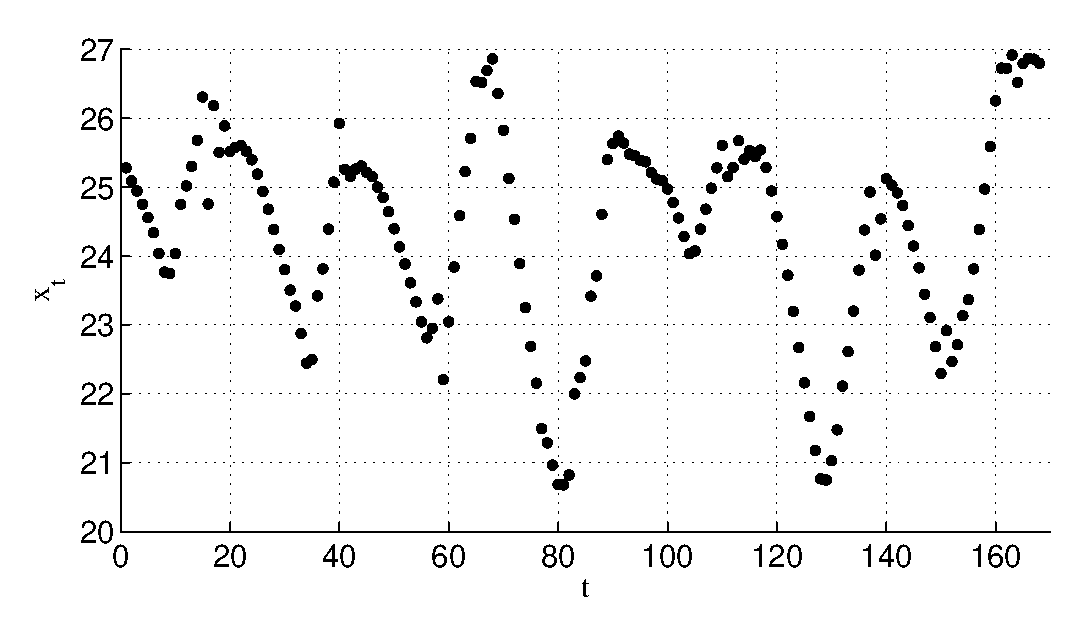
\includegraphics[scale=0.33]{CoolingSystemExample_X.eps}\\
    \begin{center}$\mathbf{X}$\end{center}
\column{0.5\textwidth}
	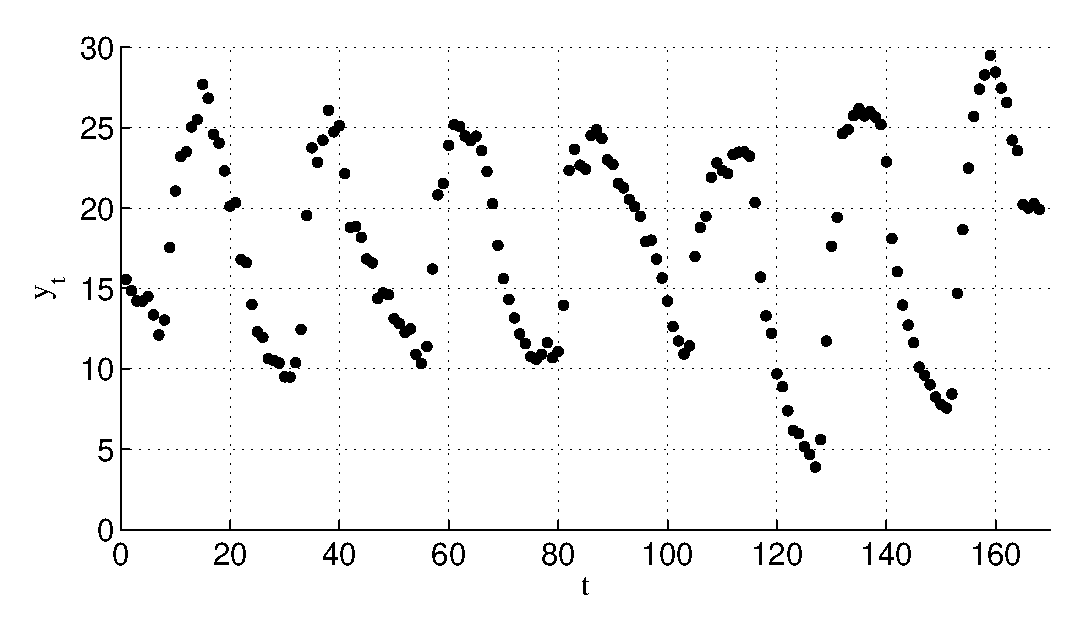
\includegraphics[scale=0.33]{CoolingSystemExample_Y.eps}\\
    \begin{center}$\mathbf{Y}$\end{center}
\end{columns}
\pause
\begin{center}\fbox{The intuitive causal inference is $\mathbf{Y}\rightarrow\mathbf{X}$.}\end{center}
\end{frame}

\begin{frame}{Cooling/Heating System Data}
\framesubtitle{ECA guess preliminaries}
An ECA guess requires several parameters be set from the data, including
\pause
\begin{itemize}
\item embedding dimension and time delay for $g_3$ (PAI)
\pause
\item cause-effect assignment and tolerance domains for $g_4$ (leaning)
\pause
\item lags for $g_5$ (cross-correlation)
\end{itemize}
\note{There are many others, including model parameters for $g_2$ (Granger) and algorithm parameters for the probability estimations in $g_1$ (transfer entropy).  These other parameters are being ignored for brevity but are explained in the paper.}
\pause
\vspace{0.1in}
The embedding dimension will be set (somewhat arbitrarily) to $E=10$ and the time delay will be $\tau=1$.
\pause
\vspace{0.1in}

The tolerance domains will be the {\em $f$-width} tolerance domains; i.e., $\pm\delta_x=f(\max(\mathbf{X})-\min(\mathbf{X}))$ and $\pm\delta_y=f(\max(\mathbf{Y})-\min(\mathbf{Y}))$.  For this example, $f=1/4$.
\pause
\vspace{0.1in}

The cause-effect assignment will be the $l$-standard assignment, but \alert{there is still the problem of determining relevant lags $l$}.

\end{frame}

\begin{frame}{Cooling/Heating System Data}
\framesubtitle{Autocorrelations}
There are autocorrelations in both time series (only 50 lags are shown),
\begin{columns}[c]
\column{0.5\textwidth}
	\includegraphics[scale=0.33]{CoolingSystemExample_autocorrX.eps}\\
    \begin{center}$\mathbf{X}$\end{center}
\column{0.5\textwidth}
	\includegraphics[scale=0.33]{CoolingSystemExample_autocorrY.eps}\\
    \begin{center}$\mathbf{Y}$\end{center}
\end{columns}
\hfill\\
The autocorrelations appear cyclic and initially drop to zero around $l=7$ for both time series.
\pause
\vspace{0.1in}

\alert{This observation will be used justify using lags of \fbox{$l=1,2,\cdots,7$} for both $g_4$ (leaning) and $g_5$ (cross-correlation).}
\note{The argument is that calculating either $g_4$ or $g_5$ for other lags would be redundant and may lead to confusing results.}
\end{frame}

\begin{frame}{Cooling/Heating System Data}
\framesubtitle{Lagged cross-correlations and leanings}
The lagged cross-correlations and leaning (using the $l$-standard assignment) can be plotted for each tested lag,
\begin{center}
\includegraphics[scale=0.50]{CoolingSystemExample_LandLCC.eps}\\
\end{center}
\pause
There are 7 different causal inferences in this plot, all of which agree except $l=7$.\pause \alert{  A single causal inference (for each tool) will be found with the algebraic mean across all the tested lags.}
\note{This is not the only approach to distilling these sets of inferences into a single inference; e.g., the maximum absolute value for each tool could be used to find a single inference.  This averaging method, however, has consistently agreed with intuition in simple examples.}
\end{frame}

\begin{frame}{Cooling/Heating System Data}
\framesubtitle{Making an ECA guess}
\tikzstyle{na} = [baseline=-.5ex]
Each of the five time series tools leads to a causal inference in the ECA guess vector,
\pause
\vspace{0.1in}

\begin{center}
\begin{tabular}{ccccc}
$T_{X\rightarrow Y}-T_{Y\rightarrow X} = -0.14$&$\Rightarrow$&$\mathbf{Y}\rightarrow\mathbf{X}$&$\Rightarrow$&\only<2-6>{$g_1 = 1$}\only<7>{\tikz[baseline]{
			\node[fill=blue!20,anchor=base] (t2)
            {$g_1=1$}}}\\
\pause
$F_{X\rightarrow Y}-F_{Y\rightarrow X}=-0.35$&$\Rightarrow$&$\mathbf{Y}\rightarrow\mathbf{X}$&$\Rightarrow$&\only<3-6>{$g_2 = 1$}\only<7>{\tikz[baseline]{
			\node[fill=blue!20,anchor=base] (t2)
            {$g_2=1$}}}\\
\pause
$C_{YX}-C_{XY}=3.1\times10^{-4}$&$\Rightarrow$&$\mathbf{Y}\rightarrow\mathbf{X}$&$\Rightarrow$&\only<4-6>{$g_3 = 1$}\only<7>{\tikz[baseline]{
			\node[fill=blue!20,anchor=base] (t2)
            {$g_3=1$}}}\\
\pause
$\langle\langle\lambda_{EC}\rangle_w\rangle=-0.20$&$\Rightarrow$&$\mathbf{Y}\rightarrow\mathbf{X}$&$\Rightarrow$&\only<5-6>{$g_4 = 1$}\only<7>{\tikz[baseline]{
			\node[fill=blue!20,anchor=base] (t2)
            {$g_4=1$}}}\\
\pause
$\langle|\rho^{xy}_l| - |\rho^{yx}_l|\rangle=0.40$&$\Rightarrow$&$\mathbf{Y}\rightarrow\mathbf{X}$&$\Rightarrow$&\only<6>{$g_5 = 1$}\only<7>{\tikz[baseline]{
			\node[fill=blue!20,anchor=base] (t2)
            {$g_5=1$}}}
\end{tabular}
\end{center}
\vspace{0.1in}
\only<7>{$\therefore$ the ECA guess is $\mathbf{Y}\rightarrow\mathbf{X}$, which agrees with intuition}
\end{frame}

\subsection{Snowfall Data}
\begin{frame}{Snowfall Data}
\framesubtitle{Time series data}
Consider a time series pair $(\mathbf{X},\mathbf{Y})$ where $\mathbf{X}$ is the mean daily temperature (in degrees Celsius) at Whistler, BC, Canada, and $\mathbf{Y}$ is the total snowfall (in centimeters) (7,753 measurements in each series)\footnotemark
\footnotetext[3]{{\tiny This data is available as part of the UCI Machine Learning Repository.  The data was recorded from July 1, 1972 to December 31, 2009.}}
\begin{columns}[c]
\column{0.5\textwidth}
	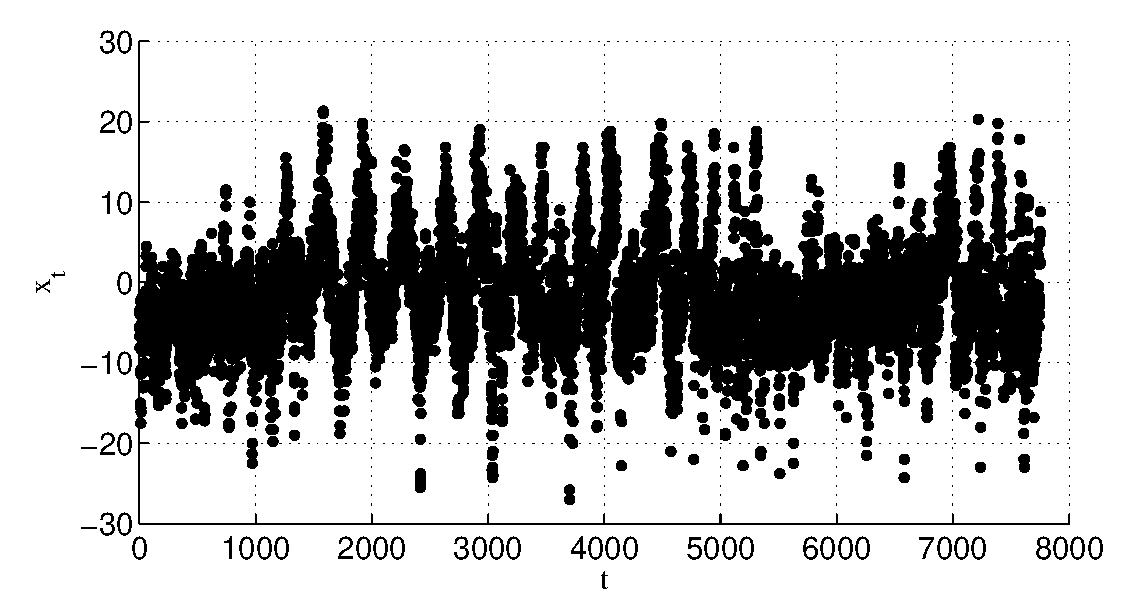
\includegraphics[scale=0.33]{WhistlerDailyExample_X.eps}\\
    \begin{center}$\mathbf{X}$\end{center}
\column{0.5\textwidth}
	\includegraphics[scale=0.33]{WhistlerDailyExample_Y.eps}\\
    \begin{center}$\mathbf{Y}$\end{center}
\end{columns}
\pause
\begin{center}\fbox{The intuitive causal inference is $\mathbf{X}\rightarrow\mathbf{Y}$.}\end{center}
\end{frame}

\begin{frame}{Snowfall Data}
\framesubtitle{ECA guess preliminaries}
The ECA guess can be made with similar parameters as the previous example,
\begin{itemize}
\item The embedding dimension will be $E=100$ with a time delay of $\tau=1$
\item The cause-effect assignment will be the $l$-standard assignment
\item The tolerance domains will be the $1/4$-width domains
\item The tested lags will be $l=1,2,\ldots,20$
\end{itemize}
\end{frame}

\begin{frame}{Snowfall Data}
\framesubtitle{Making an ECA guess}
\tikzstyle{na} = [baseline=-.5ex]
Each of the five time series tools leads to a causal inference in the ECA guess vector,
\pause
\vspace{0.1in}

\begin{center}
\begin{tabular}{ccccc}
$T_{X\rightarrow Y}-T_{Y\rightarrow X} = 2.1\times 10^{-2}$&$\Rightarrow$&$\mathbf{X}\rightarrow\mathbf{Y}$&$\Rightarrow$&\only<2-6>{$g_1 = 0$}\only<7,8>{\tikz[baseline]{
			\node[fill=blue!20,anchor=base] (t2)
            {$g_1=0$}}}\\
\pause
$F_{X\rightarrow Y}-F_{Y\rightarrow X}=-2.6\times 10^{-3}$&$\Rightarrow$&$\mathbf{Y}\rightarrow\mathbf{X}$&$\Rightarrow$&\only<3-6,8>{$g_2 = 1$}\only<7>{\tikz[baseline]{
			\node[fill=blue!20,anchor=base] (t2)
            {$g_2=1$}}}\\
\pause
$C_{YX}-C_{XY}=-3.4\times 10^{-2}$&$\Rightarrow$&$\mathbf{X}\rightarrow\mathbf{Y}$&$\Rightarrow$&\only<4-6>{$g_3 = 0$}\only<7,8>{\tikz[baseline]{
			\node[fill=blue!20,anchor=base] (t2)
            {$g_3=0$}}}\\
\pause
$\langle\langle\lambda_{EC}\rangle_w\rangle=3.7\times 10^{-2}$&$\Rightarrow$&$\mathbf{X}\rightarrow\mathbf{Y}$&$\Rightarrow$&\only<5-6>{$g_4 = 0$}\only<7,8>{\tikz[baseline]{
			\node[fill=blue!20,anchor=base] (t2)
            {$g_4=0$}}}\\
\pause
$\langle|\rho^{xy}_l| - |\rho^{yx}_l|\rangle=2.3\times 10^{-2}$&$\Rightarrow$&$\mathbf{Y}\rightarrow\mathbf{X}$&$\Rightarrow$&\only<6,8>{$g_5 = 1$}\only<7>{\tikz[baseline]{
			\node[fill=blue!20,anchor=base] (t2)
            {$g_5=1$}}}
\end{tabular}
\end{center}
\vspace{0.1in}
\only<7,8>{$\therefore$ the ECA guess is {\em undefined}}
\only<8>{
\vspace{0.1in}

\alert{The majority of the causal inferences agree with intuition.}}
\end{frame}

\section{Times series causality as data analysis}
\begin{frame}{Times series causality as data analysis}
\framesubtitle{Objections to causal studies}
Data analysis often ignores causality.
\vspace{0.2in}
\pause

Two primary objections to time series causality
\begin{enumerate}
\item \alert<3>{Correlation is not causation}
\item \alert<4>{Confounding cannot be controlled}
\end{enumerate}
\vspace{0.2in}
\pause
\alert<3>{Many different tools have been developed that go beyond correlation} and ignoring such tools means ignoring potentially useful inferences that can be drawn from the data.
\vspace{0.15in}

\pause
True, but this is an issue of defining ``causality''.  \alert<4>{Exploring} potential causal relationships within data sets can be done with \alert<4>{operational} definitions of causality.  These different causalities may provide deeper insight into the system dynamics.
\end{frame}

\begin{frame}{Times series causality as data analysis}
\framesubtitle{Expanding the notion of data analysis}
Causal analysis (either exploratory or confirmatory) can, and should, be a part of a standard data analysis approach in physics.
\end{frame}

\begin{frame}{}
\end{frame}

\begin{frame}{}
\begin{center}
BACK-UP
\end{center}
\end{frame}

\begin{frame}{Impulse with linear response}
Consider $\left\{\mathbf{X},\mathbf{Y}\right\} = \left\{\{x_t\},\{y_t\}\right\}$ where $t=0,1,\ldots,L$,
\begin{equation*}
x_t = \left\{
  \begin{array}{lr}
    2 & t = 1\\
    A\eta_t & \forall\; t\in\{t\;|\;t\neq 1 \;\mathrm{and}\; t\bmod 5 \neq 0\}\\
    2 & \forall\; t\in\{t\;|\;t\bmod 5 = 0\}
  \end{array}
\right.
\end{equation*}
and $y_t = x_{t-1} + B\eta_t$ with $y_0 = 0$, $A,B\in\mathbb{R}\ge 0$ and $\eta_t\sim\mathcal{N}\left(0,1\right)$.  Specifically, consider $L=500$, $A=0.1$, and $B=0.4$.
\begin{center}
\begin{tabular}{ccccc}
$T_{X\rightarrow Y}-T_{Y\rightarrow X} = 5.3\times 10^{-1}$&$\Rightarrow$&$\mathbf{X}\rightarrow\mathbf{Y}$&$\Rightarrow$&$g_1 = 0$\\
$F_{X\rightarrow Y}-F_{Y\rightarrow X}=4.5\times 10^{-1}$&$\Rightarrow$&$\mathbf{X}\rightarrow\mathbf{Y}$&$\Rightarrow$&$g_2 = 0$\\
$C_{YX}-C_{XY}=-8.3\times 10^{-3}$&$\Rightarrow$&$\mathbf{X}\rightarrow\mathbf{Y}$&$\Rightarrow$&$g_3 = 0$\\
$\langle\langle\lambda_{EC}\rangle_w\rangle=6.6\times 10^{-3}$&$\Rightarrow$&$\mathbf{X}\rightarrow\mathbf{Y}$&$\Rightarrow$&$g_4 = 0$\\
$\langle|\rho^{xy}_l| - |\rho^{yx}_l|\rangle=-2.8\times 10^{-3}$&$\Rightarrow$&$\mathbf{X}\rightarrow\mathbf{Y}$&$\Rightarrow$&$g_5 = 0$
\end{tabular}
\end{center}
\note{$l = 1,2,\ldots,6$}
ECA guess is $\mathbf{X}\rightarrow\mathbf{Y}$, which agrees with intuition.
\end{frame}

\begin{frame}{Cyclic driving with linear response}
Consider $\left\{\mathbf{X},\mathbf{Y}\right\} = \left\{\{x_t\},\{y_t\}\right\}$ where $t=0,1,\ldots,L$,
\begin{equation*}
x_t = a\sin(bt+c)+A\eta_t
\end{equation*}
and
\begin{equation*}
y_t = x_{t-1} + B\eta_t
\end{equation*}
with $y_0 = 0$, $A\in[0,1]$, $B\in[0,1]$, $\eta_t\sim\mathcal{N}\left(0,1\right)$, and with the amplitude $a$, the frequency $b$, and the phase $c$ all in the appropriate units.  Specifically, consider $L=500$, $A=0.1$, $B=0.4$, $a=b=1$, and $c=0$.  
\begin{center}
\begin{tabular}{ccccc}
$T_{X\rightarrow Y}-T_{Y\rightarrow X} = 1.9\times 10^{-1}$&$\Rightarrow$&$\mathbf{X}\rightarrow\mathbf{Y}$&$\Rightarrow$&$g_1 = 0$\\
$F_{X\rightarrow Y}-F_{Y\rightarrow X}=2.1\times 10^{-1}$&$\Rightarrow$&$\mathbf{X}\rightarrow\mathbf{Y}$&$\Rightarrow$&$g_2 = 0$\\
$C_{YX}-C_{XY}=-9.8\times 10^{-3}$&$\Rightarrow$&$\mathbf{X}\rightarrow\mathbf{Y}$&$\Rightarrow$&$g_3 = 0$\\
$\langle\langle\lambda_{EC}\rangle_w\rangle=3.9\times 10^{-3}$&$\Rightarrow$&$\mathbf{X}\rightarrow\mathbf{Y}$&$\Rightarrow$&$g_4 = 0$\\
$\langle|\rho^{xy}_l| - |\rho^{yx}_l|\rangle=-2.9\times 10^{-2}$&$\Rightarrow$&$\mathbf{X}\rightarrow\mathbf{Y}$&$\Rightarrow$&$g_5 = 0$
\end{tabular}
\end{center}
\note{$l = 1,2,\ldots,20$}
ECA guess is $\mathbf{X}\rightarrow\mathbf{Y}$, which agrees with intuition.
\end{frame}

\begin{frame}{Cyclic driving with non-linear response}
Consider$\left\{\mathbf{X},\mathbf{Y}\right\} = \left\{\{x_t\},\{y_t\}\right\}$ where $t=0,1,\ldots,L$,
\begin{equation*}
x_t = a\sin(bt+c)+A\eta_t
\end{equation*}
and
\begin{equation*}
y_t = Bx_{t-1}\left(1-Cx_{t-1}\right)+D\eta_t,
\end{equation*}
with $y_0 = 0$, with $A,B,C,D\in[0,1]$, $\eta_t\sim\mathcal{N}\left(0,1\right)$, and with the amplitude $a$, the frequency $b$, and the phase $c$ all in the appropriate units given $t=0,f\pi,2f\pi,3f\pi,\ldots,6\pi$ with $f=1/30$, which implies $L=181$.  Specifically, consider $A=0.1$, $B=0.3$, $C=0.4$, $D=0.5$, $a=b=1$, and $c=0$.
\begin{center}
\begin{tabular}{ccccc}
$T_{X\rightarrow Y}-T_{Y\rightarrow X} =2.7\times 10^{-1}$&$\Rightarrow$&$\mathbf{X}\rightarrow\mathbf{Y}$&$\Rightarrow$&$g_1 = 0$\\
$F_{X\rightarrow Y}-F_{Y\rightarrow X}=2.6\times 10^{-1}$&$\Rightarrow$&$\mathbf{X}\rightarrow\mathbf{Y}$&$\Rightarrow$&$g_2 = 0$\\
$C_{YX}-C_{XY}=-1.8\times 10^{-3}$&$\Rightarrow$&$\mathbf{X}\rightarrow\mathbf{Y}$&$\Rightarrow$&$g_3 = 0$\\
$\langle\langle\lambda_{EC}\rangle_w\rangle=8.4\times 10^{-3}$&$\Rightarrow$&$\mathbf{X}\rightarrow\mathbf{Y}$&$\Rightarrow$&$g_4 = 0$\\
$\langle|\rho^{xy}_l| - |\rho^{yx}_l|\rangle=-6.8\times 10^{-2}$&$\Rightarrow$&$\mathbf{X}\rightarrow\mathbf{Y}$&$\Rightarrow$&$g_5 = 0$
\end{tabular}
\end{center}
\note{$l=1,2,\ldots,20$}
ECA guess is $\mathbf{X}\rightarrow\mathbf{Y}$, which agrees with intuition.
\end{frame}

\begin{frame}{Coupled logistic map}
Consider $\left\{\mathbf{X},\mathbf{Y}\right\} = \left\{\{x_t\},\{y_t\}\right\}$ where $t=0,1,\ldots,L$,
\begin{equation*}
x_t = x_{t-1}\left(r_x-r_x x_{t-1}-\beta_{xy} y_{t-1}\right)
\end{equation*}
and
\begin{equation*}
y_t = y_{t-1}\left(r_y-r_y y_{t-1}-\beta_{yx} x_{t-1}\right)
\end{equation*}
where the parameters $r_x,r_y,\beta_{xy},\beta_{yx}\in\mathbb{R}\ge 0$.  Specifically, consider $L=500$, $\beta_{xy} = 0.5$, $\beta_{yx} = 1.5$, $r_x = 3.8$, and $r_y = 3.2$ with initial conditions $x_0 = y_0 = 0.4$.
\begin{center}
\begin{tabular}{ccccc}
$T_{X\rightarrow Y}-T_{Y\rightarrow X} =4.9\times 10^{-1}$&$\Rightarrow$&$\mathbf{X}\rightarrow\mathbf{Y}$&$\Rightarrow$&$g_1 = 0$\\
$F_{X\rightarrow Y}-F_{Y\rightarrow X}=5.4\times 10^{-1}$&$\Rightarrow$&$\mathbf{X}\rightarrow\mathbf{Y}$&$\Rightarrow$&$g_2 = 0$\\
$C_{YX}-C_{XY}=-3.9\times 10^{-3}$&$\Rightarrow$&$\mathbf{X}\rightarrow\mathbf{Y}$&$\Rightarrow$&$g_3 = 0$\\
$\langle\langle\lambda_{EC}\rangle_w\rangle=2.7\times 10^{-1}$&$\Rightarrow$&$\mathbf{X}\rightarrow\mathbf{Y}$&$\Rightarrow$&$g_4 = 0$\\
$\langle|\rho^{xy}_l| - |\rho^{yx}_l|\rangle=-2.6\times 10^{-1}$&$\Rightarrow$&$\mathbf{X}\rightarrow\mathbf{Y}$&$\Rightarrow$&$g_5 = 0$
\end{tabular}
\end{center}
\note{$l=1,2,\ldots,4$}
ECA guess is $\mathbf{X}\rightarrow\mathbf{Y}$, which agrees with intuition.
\end{frame}

\end{document}
